% vim: set expandtab tabstop=4 shiftwidth=4 textwidth=80:

\documentclass{article}
\usepackage[inner=2.5cm,outer=2.5cm,bottom=1.8cm,top=1.8cm]{geometry}
\usepackage{graphicx}% Include figure files
\graphicspath{ {./graphics/} }
\usepackage{caption}
\usepackage{subcaption}
\usepackage{numprint} % rounds numbers in tables
\npdecimalsign{.}
\nprounddigits{5}
\captionsetup{justification=centering}
\usepackage{wrapfig}
\usepackage{tabu} % for changing individual row fonts
\usepackage{amssymb, amsmath}
\usepackage[mathscr]{euscript}
\usepackage{dsfont}

% for citing things
\usepackage[hyphens]{url}
\usepackage[bookmarks]{hyperref}
%\usepackage{graphicx}
%\usepackage{verbatim}
\hypersetup{
colorlinks,
citecolor=black,
filecolor=black,
linkcolor=black,
urlcolor=black
}
\usepackage{cite}

% nicely written chi
\def\Chi{\raisebox{2pt}{$\chi$}}

%% new column table for tabu to center paragraph cells
% http://tug.org/mail-archives/texhax/2007-March/008042.html
\usepackage{array}
\newcolumntype{C}{>{\centering\arraybackslash}m{2.8cm}} 

% to thicked table lines
\usepackage{booktabs}

% make rows in tables wider
\renewcommand{\arraystretch}{1.4}% Wider

\title{Multi-layer auto-encoders \\
    \large{a CS221 artificial intelligence project}}
    \author{
    Charles Celerier \\
    Computer Science \\
    Stanford \\
    cceleri@cs.stanford.edu
  \and
    Bill Chickering \\
    Computer Science \\
    Stanford \\
    chickering@cs.stanford.edu
}

\begin{document}

\maketitle

This is a short introduction.

\section{Introduction}\label{sec:introduction}

A fundamental challenge to supervised machine learning is that of feature selection. There exist many strategies for determining a set of variables derived from an original representation to accurately classify domain data. Ideally, the selected variables minimize redundant and/or irrelevant information and thereby reduce the risk of overfitting. Historically, domain experts and computer scientists have laboriously handcrafted feature sets for a variety of machine learning problems. These manually engineered features suffer from the requirements of domain expertise and a great deal of work, and therefore, might not scale well. Moreover, such feature sets can inadvertently ignore important structure in the data. These deficiencies can be addressed via unsupervised feature learning using dimension reduction techniques such as principal component anaysis (PCA) or factor analysis. Recently it was found that K-means clustering offers another straightforward method for determining an efficacious feature space (e.g. the CS221 Visual Cortex programming assigment). In this report we document a project in which unsupervised feature learning is performed using autoencoder neural networks to discover feature spaces that can be utilized by a supervised learning algorithm to effectively classify images of handwritten digits.

Our subject is the MNIST database of handwritten digits\footnote{http://yann.lecun.com/exdb/mnist/}, which includes 50,000 training and 10,000 testing images, each a 28x28 grid of real numbers between 0 and 1. It is worth mentioning that this dataset has been employed before to demonstrate feature learning with autoencoders. Indeed, the pioneering paper by Hinton {\em et al.}\ref{art:HS} that introduced the technique upon which our project is based used this dataset among others. We chose to work with the MNIST data because of its large size, simple format, and obvious classifications thereby allowing us to focus on technique.

\section{Method}\label{sec:method}

An autoencoder is a special type of neural network consisting of an input layer, an output layer, and one or more hidden layers. An autoencoder aims to approximate the identity function as closely as possible, reproducing the signals of its input layer at its output layer. By placing constraints on the network, input signals must be compressed and decompressed using optimized encodings in order to approximately reproduce the input. Such encodings can then serve as feature sets in a supervis
ed learning problem. The challenge is training such autoencoders in order to discover the optimal e
ncoding for a particular domain space.

Until recently, the standard approach to training multilayer feedforward neural networks, such as autoencoders, is to use a variation of the backpropagation algorithm. We describe this algorithm later in this report. For now, we merely point out a key feature of the backpropagation algorithm: it attempts to optimize all weights and biases of a neural network simultaneously. In the case of large networks containing multiple layers and 1000+ nodes, backpropagation following random initialization of the parametes can fail due to local minima in the objective function\ref{art:KL}. A technique pioneered by Hinton {\em et al.}\ref{art:HS} largely overcomes this challenge by "pretraining" individual restricted Boltzmann machines (RBMs), which can then be "unrolled" to form a deep, multilayer autoencoder with weights and biases that are close to optimal prior to running a backpropagation algorithm.

An RBM may be represented as a complete bipartite graph where one set corresponds to "visible" units $\nu_i$ and the other to "hidden" units $h_j$. We work with binary RBMs in which each node is either on or off. A weight $w_{ij}$ is associated with each edge that connects a visible unit $\nu_i$ to a hidden unit $h_j$. Given the state of all visible units, the probability that a hidden unit is in the "on" state is given by $\sigma\left(b_j + \sum_i{\nu_iW_{ij}}\right)$, where $\sigma (x)$ is the logistic function $1/(1 + \mathrm{exp}(-x))$ and $b_j$ is the bias associated with hidden unit $j$. By coupling the visible and hidden units in this way, an RBM models a particular statistical ensemble of unit configurations, which in our case are images. The technique of Hinton {\em et al.} "pretrains" an RBM so that it approximately models a training set.

A detailed description of the technique of Hinton {\em et al.} is beyond the scope of this report; we refer the interested reader to the original papers referenced here as well as to our provided source code. The basic idea is to model our data as a physical system. We may then borrow some statistical machinery from physics to help pretrain our RBMs. Perhaps the most fundamental of these is the {\em free energy} ascribed to each training image, given by

\begin{equation}
E(\bf{\nu}, \bf{h}) = -\sum_{i\in\mathrm{visible}}{b_i\nu_i} - \sum_{j\in\mathrm{hidden}}{b_jh_j - \sum_{i,j}{\nu_ih_jw_{ij}}.
\end{equation}
As per the Maxwell-Boltzmann distribution, the probability of a particular image is proportional to $\mathrm{exp}\left(-E(\bf{\nu}, \bf{h})\right)$. Using stochastic gradient descent to maximize the log-likelihood of our training images, along with an approximation technique known as {\em contrastive divergence} that allows us estimate an expectation over all possible unit configurations under the probability distribution modeled by an RBM, we iteratively update the biases and weights of an RBM. Once a RBM is optimized in this manner, it is straighforward to create an autoencoder with a single hidden layer by adding an output layer that simply decodes the states of the hidden layer. To construct an autoencoder with three hidden layers, we pretrain an additional RBM using the output (i.e. hidden layer) of the first RBM as input. In this way, multiple RBMs can be unrolled to form pretrained deep neural network autoencoders.

Once pretrained, an autoencoder can be fine-tuned using backprogation without fear of local minima in our objective function (i.e. the mean squared error). As with the RBM pretraining technique, the details of this classic algorithm for training neural networks are beyond this report's scope and are well documented elsewhere (an example implementation is also provided within our source code). The essence of this algorithm is to propagate the discrepancy between the autoencoder's output and its input back through the neural network, adjusting its parameters along the way.

\section{Results}\label{sec:results}

\begin{figure}[htbp!]
    \centering
    \begin{subfigure}{.45\textwidth}
        \centering
        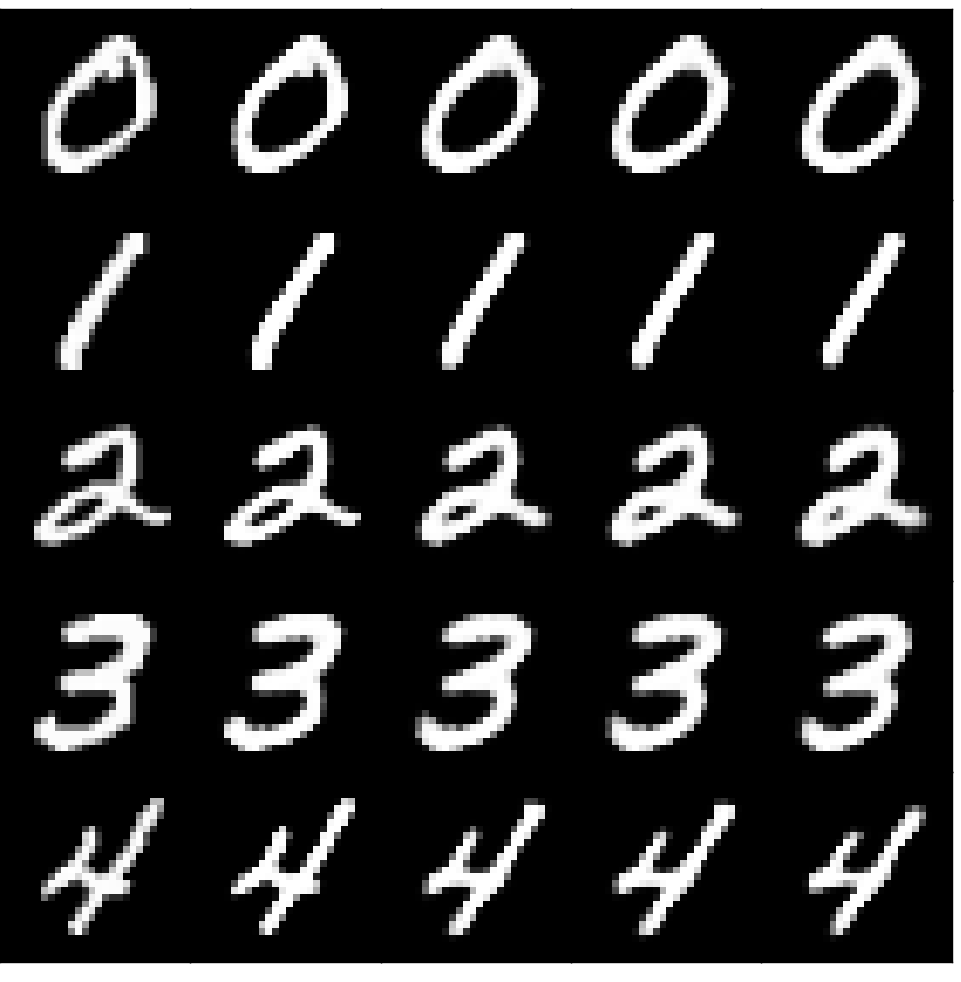
\includegraphics[width=\textwidth]{incremental_0-4.png}
        \caption{Encoding of digits $0-4$ in each layer}
        \label{fig:incremental_0-4}
    \end{subfigure}%
    \quad
    \begin{subfigure}{.45\textwidth}
        \centering
        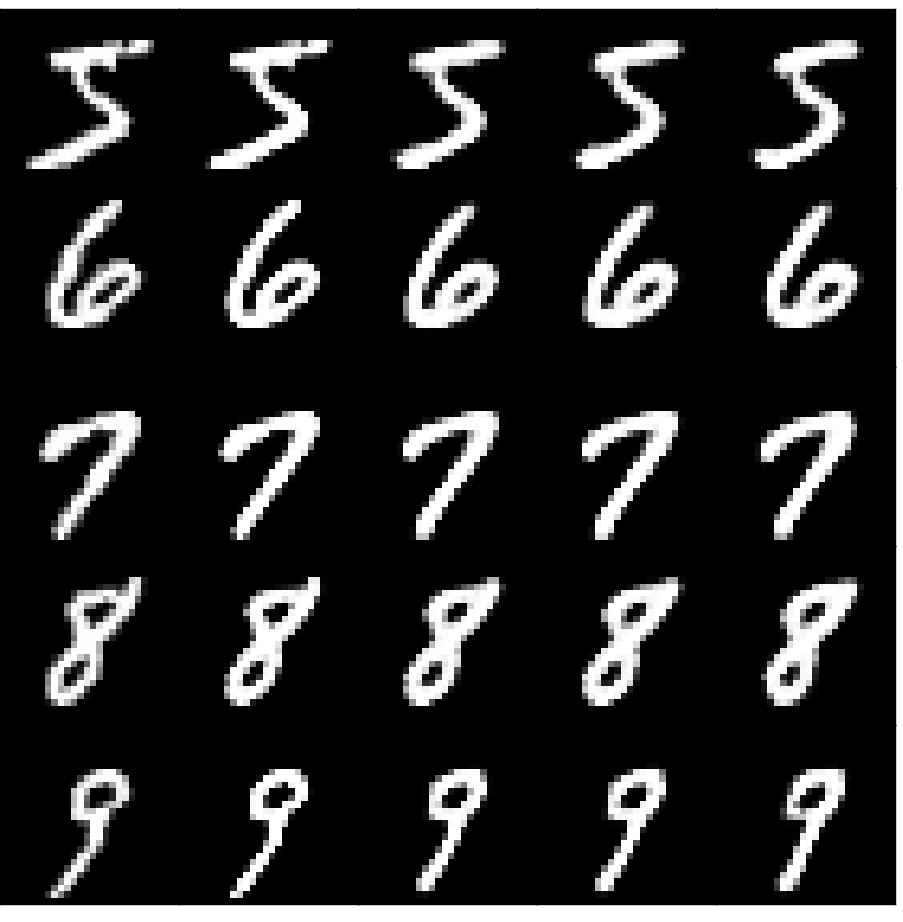
\includegraphics[width=\textwidth]{incremental_5-9.png}
        \caption{Encoding of digits $5-9$ in each layer}
        \label{fig:incremental_5-9}
    \end{subfigure}
\end{figure}

Here's an equation:

\begin{equation}
    \mathscr{C} = \frac{\sum_{q \in Q}\sum_{i=1}^{L_q}\mathds{1}\left\{click\; @\; i \wedge i \leq 16\right\}}{\sum_{q \in Q}\sum_{i=1}^{L_q}\mathds{1}\left\{i \leq 16\right\}},
\end{equation}

\section{Conclusion}\label{sec:conclusion}

\nocite{*}
\bibliography{refs}{}
\bibliographystyle{amsplain}

\end{document}

% vim: set tw=80 ts=4 sw=4 expandtab smarttab:

